\chapter{Mode Finders and Finite Difference Method}

Starting from the Maxwell's equations, without sources and in the
harmonic regime, we have:
\begin{equation}
  \left\{
  \begin{array}{ll}
    \Rot{\E} = -\imath \omega \mu_0 \H \\
    \Rot{\H} = \imath \omega \epsilon \E
  \end{array}
  \right.
\end{equation}
From the second equation we can write $\E = \frac{1}{\imath
\omega \epsilon} \Rot{\H}$ and reduce to the Helmholtz
equation for the $\H$ field:
\begin{equation} \label{eqn:helmholtz_h}
  \Rot{\frac{1}{\epsilon} \Rot{\H}} - \omega^2 \mu_0
  \H = 0
\end{equation}
The choice of using the Helmholtz equation in $\H$ instead of
$\E$ is not random: we'll see that this leads to easier and
cleaner solutions (no spurious modes and better convergence because
$\H$ is always continuous).

Where $\epsilon$ is homogeneous, we can reduce to the Laplace
equation:
\begin{equation} \label{eqn:helmholtz_decoupled}
  \Lap{\H} + \omega^2 \mu_0 \epsilon \H = 0
\end{equation}
where we have used $\Rot{\Rot{\bullet}} = \Grad{\Div{\bullet}} -
\Lap{\bullet}$ and $\Div{\H} = 0$. In Cartesian coordinates, $\H =
(H_x,H_y,H_z)$ and the Laplace equation applied to the transverse
coordinates $x$ and $y$, supposing a $z$ dependence of $e^{-\imath
  \beta z}$, becomes:
\begin{equation} \label{eqn:helmholtz_decoupled_cartesian}
  \left\{
  \begin{array}{ll}
    \pdx^2 H_x + \pdy^2 H_x + (\omega^2 \mu_0 \epsilon - \beta^2) H_x = 0 \\
    \pdx^2 H_y + \pdy^2 H_y + (\omega^2 \mu_0 \epsilon - \beta^2) H_y = 0
  \end{array}
  \right.
\end{equation}

Note that $H_x$ and $H_y$ are decoupled. Coupling between the two
transverse components only arise where $\epsilon$ is not homogeneous
and the bigger the changes in $\epsilon$ the stronger the
coupling. This can be easily seen also theoretically, where in low
index contrast devices modes are \emph{almost} TE or TM, while in high
index contrast devices they are hybrid.

The Helmholtz equation, alone, is not equivalent to the Maxwell's
equations: it does have solutions that are not solution of the
Maxwell's equations, which are called \emph{spurious solutions}. To
avoid them, a supplementary condition must be imposed: $\Div{\H} = 0$:
in fact taking the divergence of \eqref{eqn:helmholtz_h} it is clear that,
without this condition, an arbitrary field $\H$ (also non
divergenless) at zero frequency would be a solution. This would be,
obviously, non physical, because $\Div{\H} = 0$ for every frequency.

To study HIC and polarization converting devices we need a fully
vectorial mode finder.

why vectorial is better that semivectorial.

we have implemented both of them!

\begin{itemize}
\item
  effective index method -> not accurate results: we need the
  effective rix precise at $10^{-5}$ at least (because devices are about
  1 mm long)
\item
  finite difference method (or finite element method)
  \begin{itemize}
  \item
    semivectorial -> stern
  \item
    vectorial -> lusse
  \item
    comparison: chose some examples (from lusse analysis, for example)
    and compare semivectorial w/ vectorial (and w/ FIMMWAVE?)
  \end{itemize}
\end{itemize}

\section{Semivectorial Mode Solver}

Taken from \cite{stern_semivectorial}.

The semivectorial mode solver that we implemented is a very simple,
yet accurate, method, which can be used to have a first insight into
the problem, when an absolute accuracy is not needed.

Ridge waveguides like the one in the figure can be studied: the
refractive index profile precludes an analytical solution which is,
strictly speaking, fully vectorial. In fact, TE and TM polarizations
can not be distinguished, at least theoretically: this is particularly
true the higher the refractive index discontinuities are.

The semplicity of the present derives from some hypothesis on the
geometry and the physics of the problem: they are both its strenght and
its weakness, because the solution will be not only numerically but
also physically approximated with respect to the reality.

These hypothesis are:
\begin{enumerate}
\item
  the refractive index is piecewise constant, with the
  discountinuities occurring only at horizontal or vertical planes (in
  a carthesian coordinate system);
\item
  TE and TM polarizations are considered as decoupled, instead of being
  coupled into a fully vectorial solution: this hypothesis leads to
  formulate two separate eigenproblems, one for each polarization, of
  smaller dimension than the full vectorial problem, but gives
  incorrect results if high refractive index discontinuities are
  present.
\end{enumerate}

Starting from the Maxwell's equations in the frequency domain, we
have:
\begin{equation} \label{eqn:stern_maxwell}
  \left\{ \begin{array}{l}
  \Rot{\E} = -\imath \omega \mu \H \\
  \Rot{\H} = \imath \omega \epsilon \E \\
  \Div{\D} = 0 \\
  \Div{\B} = 0
  \end{array} \right.
\end{equation}
and we obtain:
$$
\Rot{\Rot{\E}} = \Grad{\Div{\E}} - \Lap{\E} = \omega^2 \epsilon \mu
\E = k^2 \E
$$
The first hypothesis leads to the first semplification: inside the
region of refractive index constantness $\Div{\E} = 0$ and the
previous equation becomes:
\begin{equation} \label{eqn:stern_helmholtz}
\Lapt{\E} + k^2 \E = \beta^2 \E
\end{equation}
where we have supposed a $z$ dependance of the $\E$ fields of the
type $e^{- \imath \beta z}$ and $\Lapt{} = \pdx^2 + \pdy^2$.

More precisely, from the third of \eqref{eqn:stern_maxwell} we can
write:
$$
\Div{\D} = \Div{(\epsilon \E)} = \DotProd{\Grad{\epsilon}}{\E} +
\epsilon \Div{\E} = 0
$$
from which we can write:
$$
\Div{\E} = \DotProd{\frac{\Grad{\epsilon}}{\epsilon}}{\E}
$$
Where $\epsilon$ is piecewise constant, $\Grad{\epsilon} = 0$ and
$\Div{\E} = 0$ is satisfied: elsewhere, this is not strictly true, but
the smaller the gradient, the smaller the refractive index
discontinuities and the less important this approximation.

Equation \eqref{eqn:stern_helmholtz} does not contain any coupling between
the $x$ and $y$ component of the $\E$ field, therefore it holds
independently for each polarization:
\begin{equation} \label{eqn:stern_helmholtz_decoupled}
\Lapt{\E} + k^2 \E = \beta^2 \E \qquad \Rightarrow \qquad
\left\{
\begin{array}{l}
  \Lapt{E_x} + k^2 E_x = \beta^2 E_x \\
  \Lapt{E_y} + k^2 E_y = \beta^2 E_y
\end{array}
\right.
\end{equation}

We use now the second hypothesis: for the TE polarization, the
electric field is $\E = (E_x,0,E_z)$ and the first equation in
\eqref{eqn:stern_helmholtz_decoupled} holds; for the TM polarization,
$\E = (0,E_y,E_z)$ and the second holds.

The Helmholtz equations \eqref{eqn:stern_helmholtz_decoupled} must now
be discretized somehow, to be able to solve it on a
computer. Discretization is done substituting the second order
derivatives by finite differences on an orthogonal grid, like the one
in the figure. Each internal interface is placed half-way between
adjacent grid lines and each internal grid point is placed at the
center of a rectangular cell of constant refractive index. Refractive
index changes are only allowed at cell boundaries.

On the domain boundaries, we can impose different conditions:
\begin{itemize}
\item
  \emph{Perfect Electric Conductor}: null tangential $\E$ and
  $\partial_n \E$, with $n$ direction normal to the wall;
\item
  \emph{Perfect Magnetic Conductor}: null orthogonal $\E$ and
  $\partial_t \E$, with $t$ direction tangent to the wall;
\item
  \emph{Perfectly Matched Layers} or \emph{Transparent Boundary
  Conditions} to simulate free space.
\end{itemize}

For the TE polarization, the discretization translates the second
order devivatives to:
$$
\begin{array}{l}
h_x^2 (\pdx^2 E_x)^{(P)}_{r,s} \simeq 2 K^{(L)}_{r-1,s} E_{r-1,s} - [2 +
  (K^{LP}_{r,s} - K^{L}_{r-1,s}) + (K^{RP}_{r,s} - K^{R}_{r+1,s})]
E_{r,s} + 2 K^{(R)}_{r+1,s} E_{r+1,s} \\
h_y^2 (\pdy^2 E_x)^{(P)}_{r,s} \simeq E_{r,s-1} - 2 E_{r,s} + E_{r,s+1}
\end{array}
$$
Note that the $E_x$ component is continuous across horizontal
interfaces and discountinuous across vertical interfaces: this is the
reason for the factors $K$, which are:
$$
\begin{array}{l}
K^{(R)}_{r+1,s}  = k^2_{r+1,s} / (k^2_{r,s} + k^2_{r+1,s}) \\
K^{(RP)}_{r+1,s} = k^2_{r,s}   / (k^2_{r,s} + k^2_{r+1,s}) \\
K^{(L)}_{r-1,s}  = k^2_{r-1,s} / (k^2_{r-1,s} + k^2_{r,s}) \\
K^{(LP)}_{r+1,s} = k^2_{r,s}   / (k^2_{r-1,s} + k^2_{r,s})
\end{array}
$$
Substitution in \ref{eqn:stern_helmholtz_decoupled} and letting
$\Matrix{E}_{TE}$ being the column vector with all the $E_x$ values, one
for each node of the grid, we can write the matricial eigenvalue
equation:
$$
\Matrix{A}_{TE} \Matrix{E}_{TE} = \beta^2_{TE} \Matrix{E}_{TE}
$$
The ordering in which the $E_x$ values are stored in the
$\Matrix{E}_{TE}$ vector is chosen to reduce the spectrum of the
matrix $\Matrix{A}_{TE}$, for an easier iterative solution.

A very similar reasoning can be done on the TM polarization, for which
the $E_y$ component is continuous across vertical interfaces and
discountinuous across horizontal interfaces. We end up with a
matricial equation of the kind:
$$
\Matrix{A}_{TM} \Matrix{E}_{TM} = \beta^2_{TM} \Matrix{E}_{TM}
$$

\section{Vectorial Mode Solver} \label{sec:vectorial_mode_solver}

Taken from \cite{lusse_analysis}.

We have also implemented a fully vectorial mode finder. As said
before, this is necesarry if we are interested in studying \emph{High
  Index Contrast} (HIC) or polarization converting devices: in fact,
semivectorial algorithms do not take into account polarization
information.

The algorithm chosen is the one presented in \cite{lusse_analysis},
that we are going to describe here. It is based on the Finite
Difference approach and, with a proper formulation of the problem and
of the boundary conditions, it ensures the absence of spurious
modes. It has also been proven to achieve a considerable precision on
the computed effective index, which is necessary on today's designs:
millimiters long devices are quite common and a variation of the
effective index as small as $10^{-5}$ at optical frequencies ($\lambda
= 1.5 \mu m$) can make all the difference.

Consider a $z$-invariant waveguide and discretize its cross section
$xy$ with a finite difference mesh. Finally, suppose the magnetic
field $\H$ attached to the nodes of the mesh and the refractive index
constant inside each rectangle of the mesh: discontinuities can only
occur at the grid points. Therefore, inside each rectangle of the
mesh, the decoupled version of the Helmholtz equation
\ref{eqn:helmholtz_decoupled_cartesian} holds. In its discretized
form, for both $H_x$ and $H_y$, it reads:
\begin{eqnarray} \label{eqn:helmholtz_expansion}
  \frac{2 H_W}{w^2} - \frac{2 H_P}{w^2} + \frac{2}{w} \pdx H|_w +
  \frac{2 H_N}{w^2} - \frac{2 H_P}{w^2} + \frac{2}{w} \pdx H|_n +
  \epsilon_1 k^2 H_P = \beta^2 H_P \label{eqn:helmholtz_discretized_nw} \\
  \frac{2 H_W}{w^2} - \frac{2 H_P}{w^2} + \frac{2}{w} \pdx H|_w +
  \frac{2 H_S}{w^2} - \frac{2 H_P}{w^2} + \frac{2}{w} \pdx H|_s +
  \epsilon_2 k^2 H_P = \beta^2 H_P \label{eqn:helmholtz_discretized_sw} \\
  \frac{2 H_E}{w^2} - \frac{2 H_P}{w^2} + \frac{2}{w} \pdx H|_e +
  \frac{2 H_S}{w^2} - \frac{2 H_P}{w^2} + \frac{2}{w} \pdx H|_s +
  \epsilon_3 k^2 H_P = \beta^2 H_P \label{eqn:helmholtz_discretized_se} \\
  \frac{2 H_E}{w^2} - \frac{2 H_P}{w^2} + \frac{2}{w} \pdx H|_e +
  \frac{2 H_N}{w^2} - \frac{2 H_P}{w^2} + \frac{2}{w} \pdx H|_n +
  \epsilon_4 k^2 H_P = \beta^2 H_P \label{eqn:helmholtz_discretized_ne}
\end{eqnarray}
where we have expanded $H_W$ in Taylor serie:
$$
H_W = H_P + \pdx H|_w (-w) + \frac{1}{2} \pdx^2 H|_w (-w)^2 + \BigO{w^3}
$$
to express the second order derivative in $x$. Analogous expressions
holds for $H_S$, $H_E$, $H_N$ and $\pdy^2$. Note that the first order
derivatives are not discretized: the reason will be clear after the
discussion about the boundary conditions.

The divergenless condition of $\H$ is imposed through the boundary
conditions. $H_z$ and $E_z$ are both continuos every where on the $xy$
plane; the divergenceless condition for $\H$ becomes:
\begin{equation} \label{eqn:continuity_hz}
\Div{\H} = 0 \qquad \Rightarrow \qquad H_z = \frac{1}{\imath
  \beta} \{ \pdx H_x + \pdy H_y \}
\end{equation}
and, from the second of Maxwell's equations:
\begin{equation} \label{eqn:continuity_ez}
  \Rot{\H} = \imath \omega \epsilon \E \qquad \Rightarrow \qquad E_z =
  \frac{1}{\imath \omega \epsilon} \{ \pdx H_y - \pdy H_x \}
\end{equation}
Discontinuities of $\epsilon$ can only occur on gridpoints of the
mesh, so the boundaries between two different values of $\epsilon$ can be:
\begin{enumerate}
\item
  horizontal boundaries: on which $H_x$ and $H_z$ are continuous, and
  \ref{eqn:continuity_hz} becomes:
  $$
  \dy H_y|_n = \dy H_y|_s
  $$
  while, \ref{eqn:continuity_ez} becomes:
  $$
  \epsilon_n \dy H_x|_s - \epsilon_s \dy H_x|_n = (\epsilon_n -
  \epsilon_s) \dy H_x
  $$
\item
  vertical boundaries: on which $H_y$ and $H_z$ are continuous, and
  \ref{eqn:continuity_hz} and \ref{eqn:continuity_ez} become,
  respectively:
  $$
  \pdx H_x|_w = \pdx H_x|_e
  $$
  and
  $$
  \epsilon_e \pdx H_y|_w - \epsilon_w \pdx H_y|_e = (\epsilon_e -
  \epsilon_w) \pdx H_y
  $$
\end{enumerate}

With these four boundary conditions and the equations
\ref{eqn:helmholtz_expansion} the requested coupled differential
equations in $H_x$ and $H_y$ can be obtained. Just note that, for the
$H_x$ component, multiplying the first equation in
\ref{eqn:helmholtz_expansion} by $\epsilon_2 n/2$ and summing it to
the second multiplied by $\epsilon_1 s/2$ we obtain the left hand side
of the second boundary condition. Similar arithmetic manipulations
can be done, to obtain all the terms in the boundary conditions and
eliminate the first order derivative in \ref{eqn:helmholtz_expansion}.
Finally, two coupled equations in $H_x$ and $H_y$ can be written, in
the form:
\begin{equation}
  \left\{
  \begin{array}{l}
    a_{xxW} H_{xW} + a_{xxE} H_{xE} + a_{xxN} H_{xN} + a_{xxS} H_{xW}
    + a_{xxP} H_{xP} + \\
    a_{xyW} H_{yW} + a_{xyP} H_{yP} + a_{xyE} H_{yE} = \beta^2 H_{xP} \\
    a_{yyW} H_{yW} + a_{yyE} H_{yE} + a_{yyN} H_{yN} + a_{yyS} H_{yW}
    + a_{yyP} H_{yP} + \\
    a_{yxW} H_{xW} + a_{yxP} H_{xP} + a_{yxE} H_{xE} = \beta^2 H_{yP}
  \end{array}
  \right.
\end{equation}
In a more compact matricial form:
\begin{equation}
  \Matrix{A} \Matrix{H} = \left[
    \begin{array}{cc}
      A_{xx} & A_{xy} \\
      A_{yx} & A_{yy}
    \end{array} \right]
  \left[ \begin{array}{c}
      H_x \\
      H_y
    \end{array} \right] = \beta^2
  \left[ \begin{array}{c}
      H_x \\
      H_y
    \end{array} \right] = \beta^2 \Matrix{H}
\end{equation}
where $\Matrix{A_{ij}}$ contain the coefficient $a_{ij}$, $i,j =
x,y$. Note that the coupling between $H_x$ and $H_y$ is caused by the
elements of the off-diagonal matrices $\Matrix{A}_{xy}$ and
$\Matrix{A}_{yx}$: in semivectorial algorithms or for homogeneous
regions, they are the zero.

\section{Examples}

As an example of a typical device that can be studied with the present
mode solvers, consider the rib waveguide presented in \cite{lohmeyer_wmm}.

The domain is shown in \figref{fig:rib}, where: $n_s = 3.34$, $n_f =
3.44$, $n_c = 1.0$, $w = 2 \mu m$, $h = 1.1 \mu m$ and $t = 0.2 \mu m$.

\begin{figure}[htbp]
  \begin{center}
    \resizebox{4cm}{!}{\input{pics/rib.pdf_t}}
  \end{center}
  \caption{Rib waveguide profile, taken from \cite{lohmeyer_wmm}.}
  \label{fig:rib}
\end{figure}

Results are shown for both the algorithms, semivectorial and fully
vectorial, in \figref{fig:wmm1_stern} and \figref{fig:wmm1_lusse}
respectively. The first four guided modes are plotted, two TE and two
TM. The accordance between the two algorithms, in this case, is very
good (see \tabref{tab:wmm1}), within $0.02\%$ and they agree with the
results reported in \cite{lohmeyer_wmm}.

\begin{table}[htbp]
  \begin{center}
    \begin{tabular}{|*{5}{c|}}
      \hline
      & $TE_1$ & $TE_2$ & $TM_1$ & $TM_2$ \\
      \hline
      Semivectorial & 3.387372 & 3.331755 & 3.388132 & 3.327159 \\
      Vectorial & 3.388086 & 3.325017 & 3.387138 & 3.331010 \\
      \hline
    \end{tabular}
  \end{center}
  \caption{Effective index for the first four modes of the rib
    waveguide in \figref{fig:rib}, computed by both the semivectorial
    and vectorial mode solver.}
  \label{tab:wmm1}
\end{table}

The mode profiles obtained are reported in \figref{fig:wmm1_stern} for
the semivectorial algorithm and in \figref{fig:wmm1_lusse} for the
vectorial one. Special care has been taken to make the domain large
enough so that the guided modes are far from the boundaries: in fact,
no PMLs are present.

\begin{figure}[htbp]
  \begin{center}
    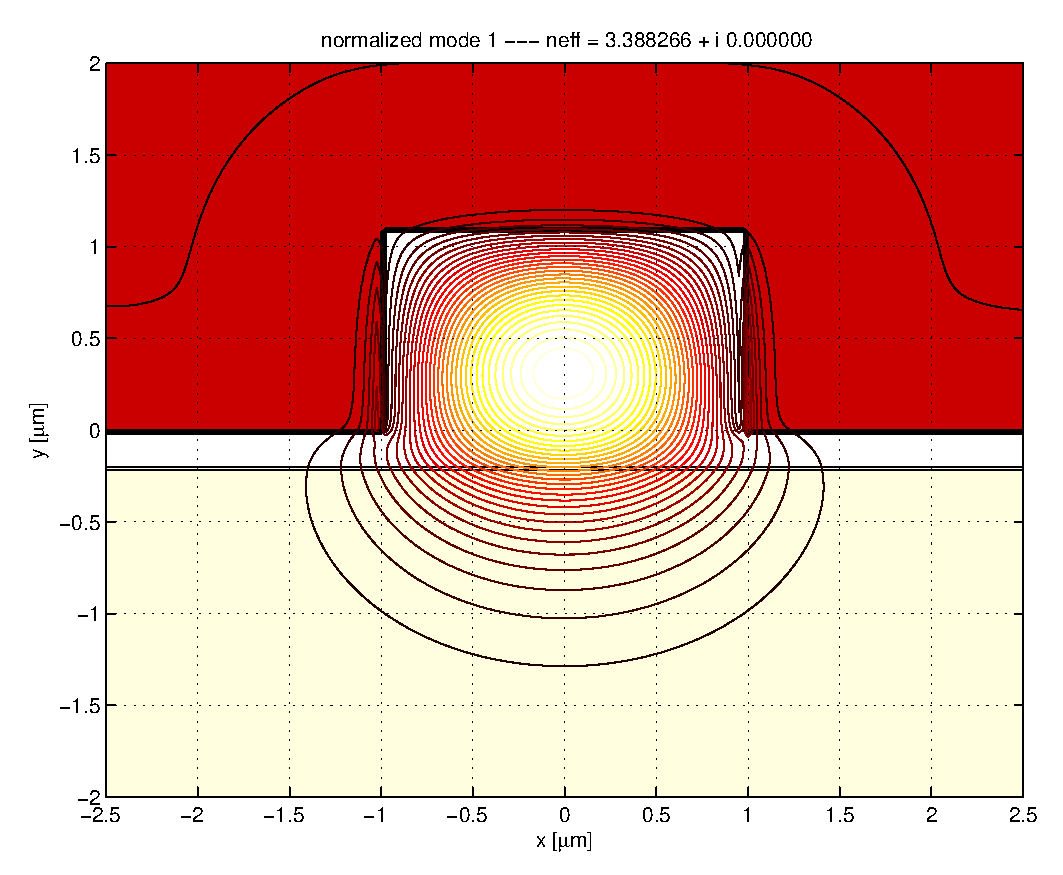
\includegraphics[width=5cm]{pics/wmm01_stern_TE1}
    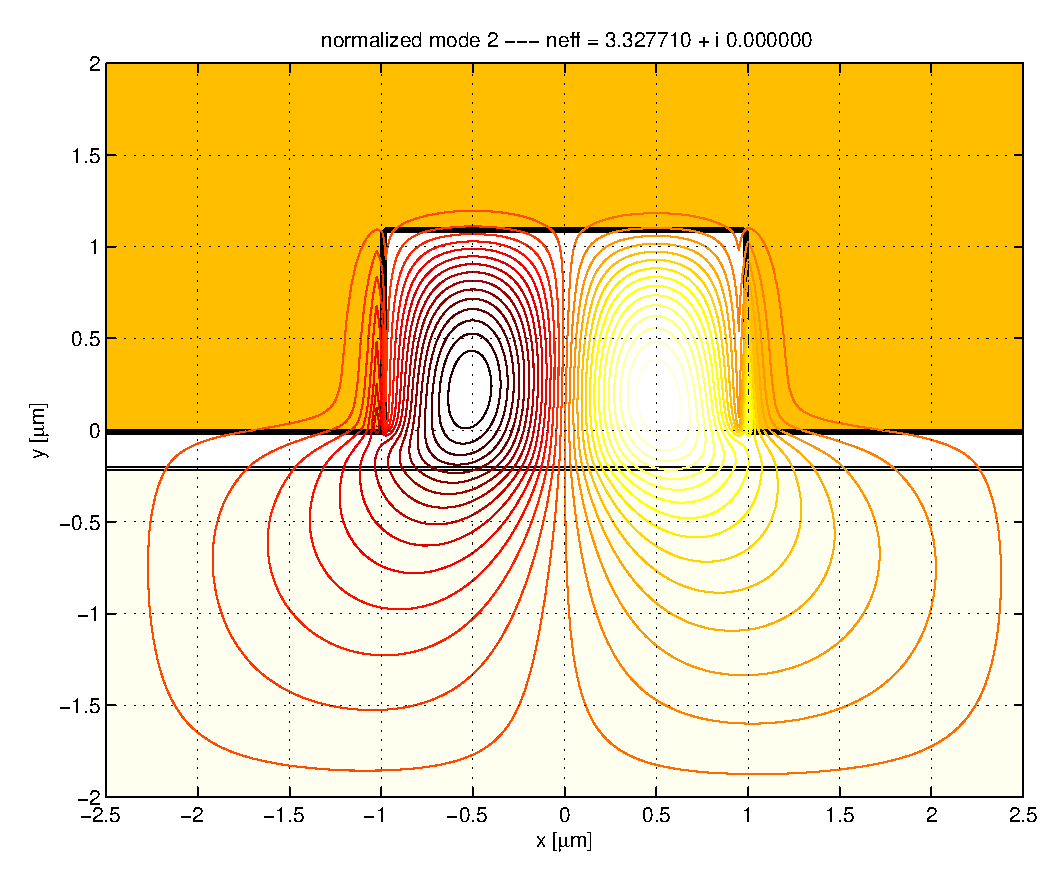
\includegraphics[width=5cm]{pics/wmm01_stern_TE2}
    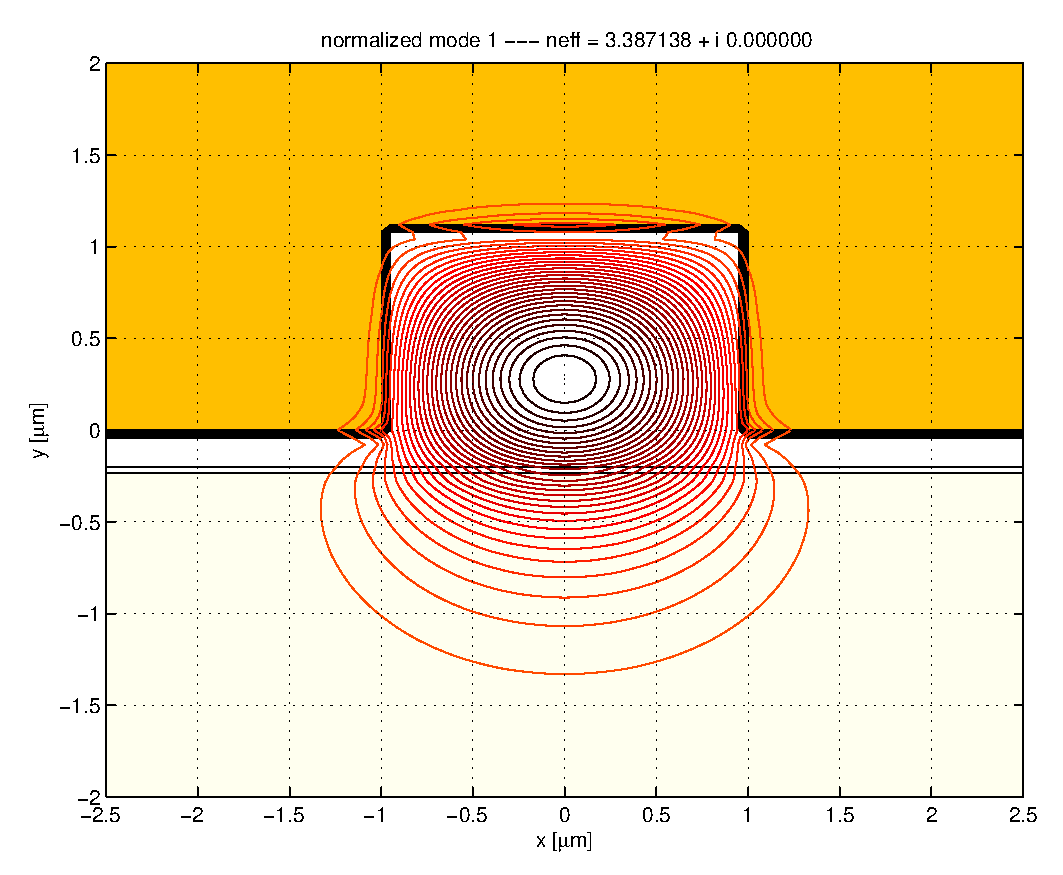
\includegraphics[width=5cm]{pics/wmm01_stern_TM1}
    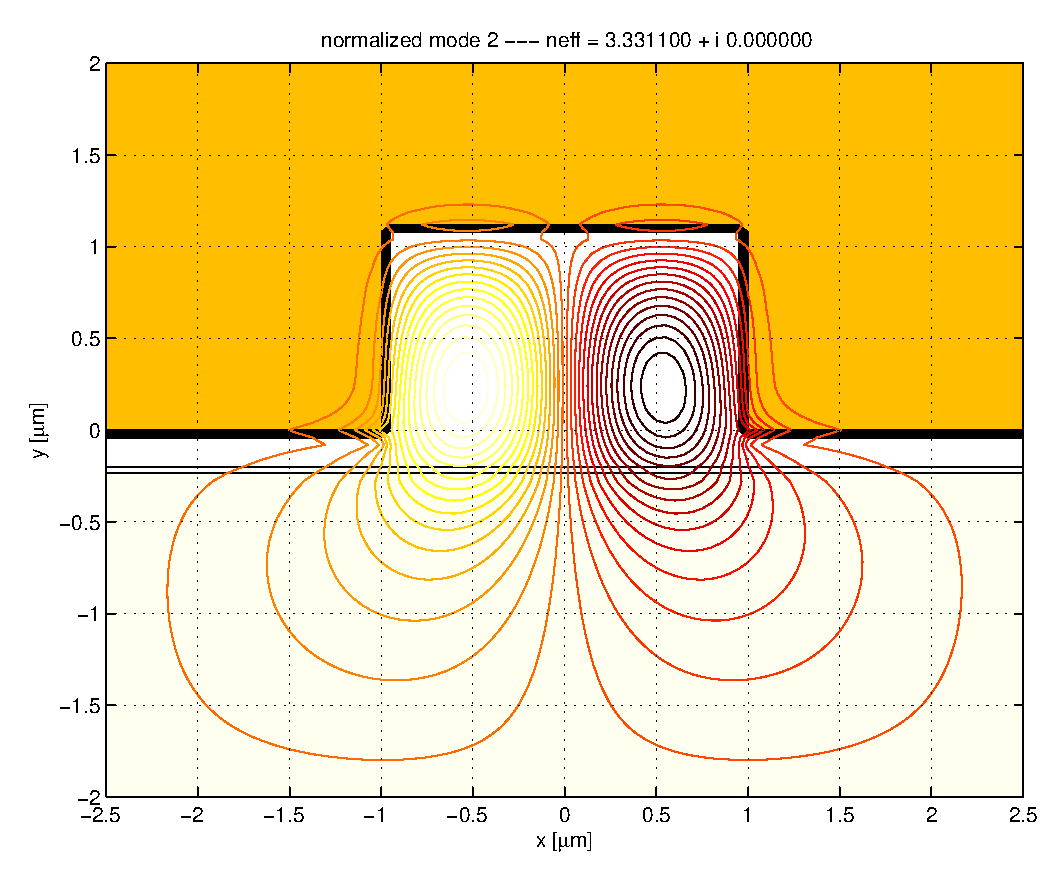
\includegraphics[width=5cm]{pics/wmm01_stern_TM2}
  \end{center}
  \caption{wmm 1 stern.}
  \label{fig:wmm1_stern}
\end{figure}  

\begin{figure}[htbp]
  \begin{center}
    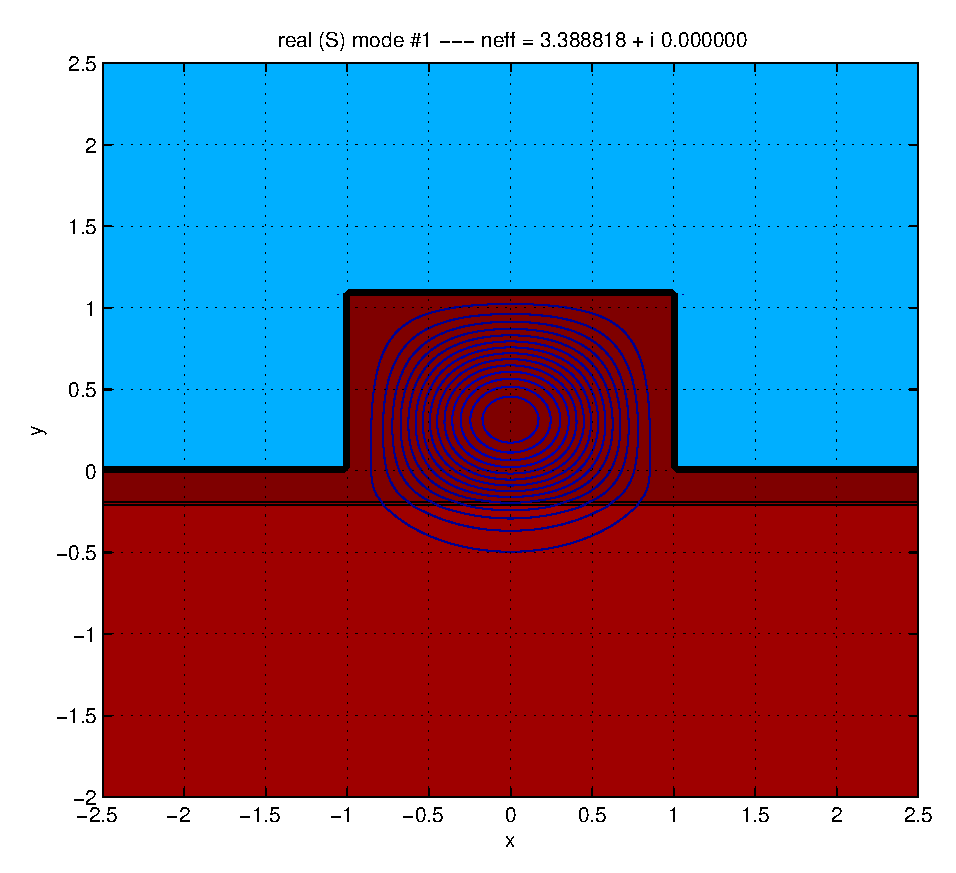
\includegraphics[width=5cm]{pics/wmm01_lusse_1}
    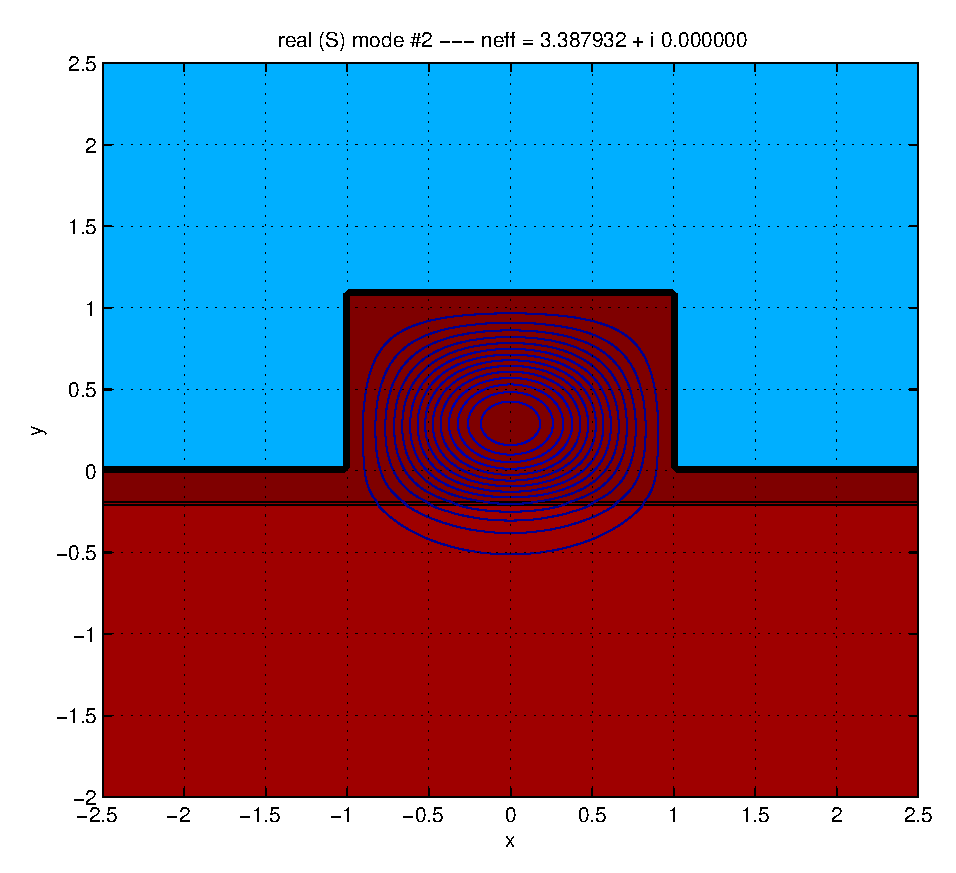
\includegraphics[width=5cm]{pics/wmm01_lusse_2}
    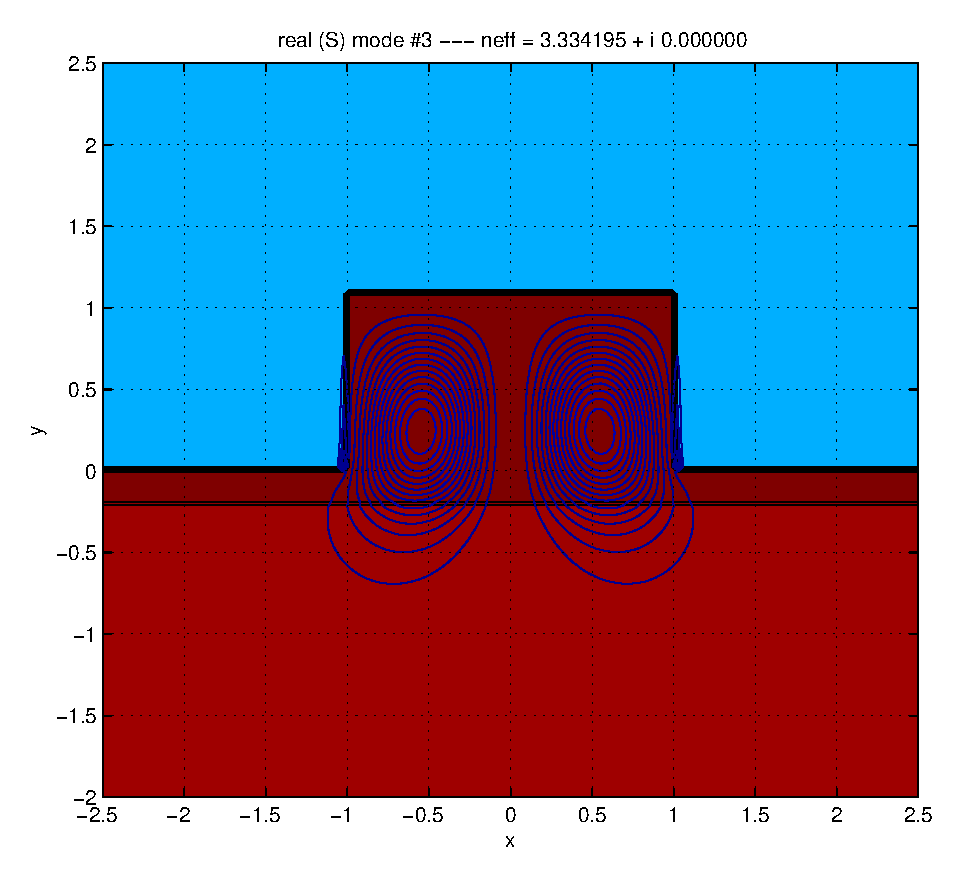
\includegraphics[width=5cm]{pics/wmm01_lusse_3}
    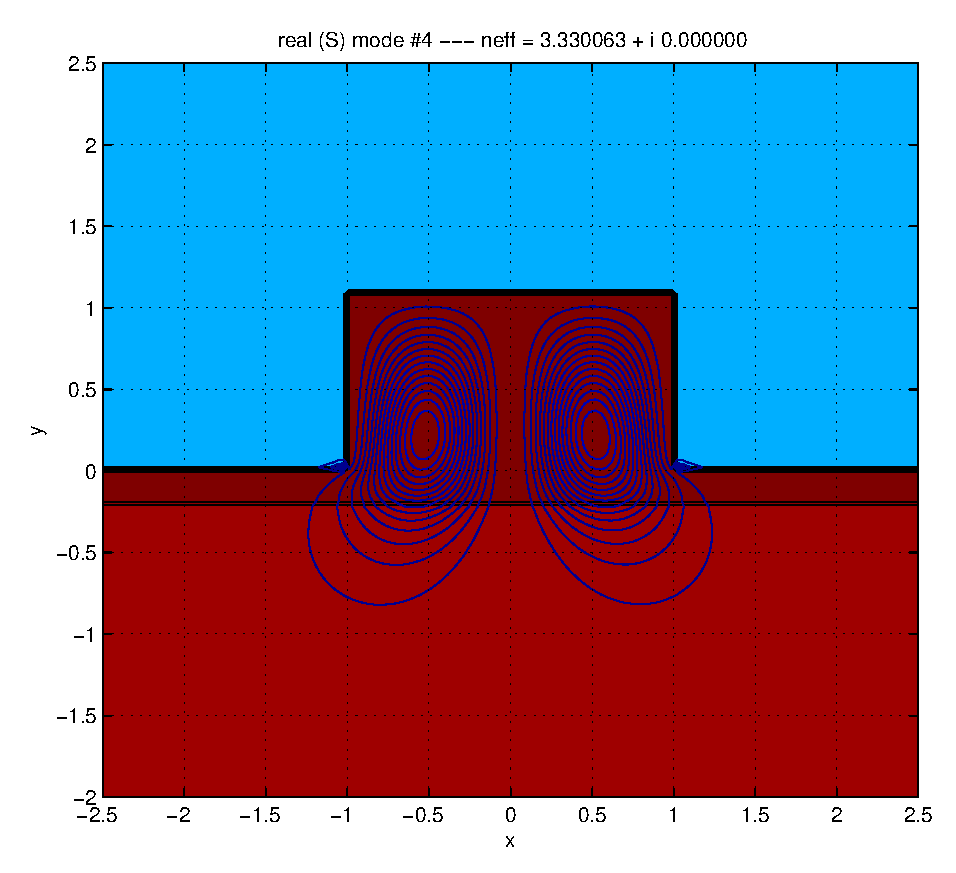
\includegraphics[width=5cm]{pics/wmm01_lusse_4}
  \end{center}
  \caption{wmm 1 lusse.}
  \label{fig:wmm1_lusse}
\end{figure}  

In this example, agreement between the semivectorial and the vectorial
mode solver is very good: it could lead to think that the two
algorithms are equivalent and the results are always similar. It is
not true. It only happens because for the particular choice of the
waveguide studied (a rib waveguide) the guided modes, even if not
purely TE nor TM, are strongly quasi-TE and quasi-TM, with very
small longitudianal $E_z$ and $H_z$ components: ignoring them is a
very little approximation.

In the next example, a waveguide, where a fully vectorial mode solver
is needed, is studied. The device is shown in \figref{fig:plabs}. It
is a buried rectangular waveguide of $Si$ ($n_{core} = 3.45$) in $SiO_2$
($n_{cladding} = 1.445$), with $w = 500 nm$ and $h = 220 nm$.

\begin{figure}[htbp]
  \begin{center}
    \resizebox{5cm}{!}{\input{pics/plabs.pdf_t}}
  \end{center}
  \caption{Buried rectangular waveguide profile.}
  \label{fig:plabs}
\end{figure}

\tabref{tab:plabs} shows the results obtained with the two
algorithms. They differ greatly. In particular, the results given by
the semivectorial mode solver are definitely inaccurate: it predicts
that all the four modes are guided, while only the first two TE and
the first TM modes are \cite{plabs}, as correctly predicted by the
vectorial mode solver.

\begin{table}[htbp]
  \begin{center}
    \begin{tabular}{|*{5}{c|}}
      \hline
      & $TE_1$ & $TE_2$ & $TM_1$ & $TM_2$ \\
      \hline
      Semivectorial & 2.633596 & 2.263625 & 2.532738 & 1.976528 \\
      Vectorial & 2.446252 & 1.525369 & 1.800634 & 1.333947 \\
      \hline
    \end{tabular}
  \end{center}
  \caption{Effective index for the first four modes of the buried
    rectangular waveguide in \figref{fig:plabs}, computed by both the
    semivectorial and vectorial mode solver. Note that the $TM_2$ mode
    is guided for the semivectorial mode solver and not guided for the
    vectorial: the semivectorial is wrong.}
  \label{tab:plabs}
\end{table}

\begin{figure}[htbp]
  \begin{center}
    \subfigure[First TE mode: magnetic field.]{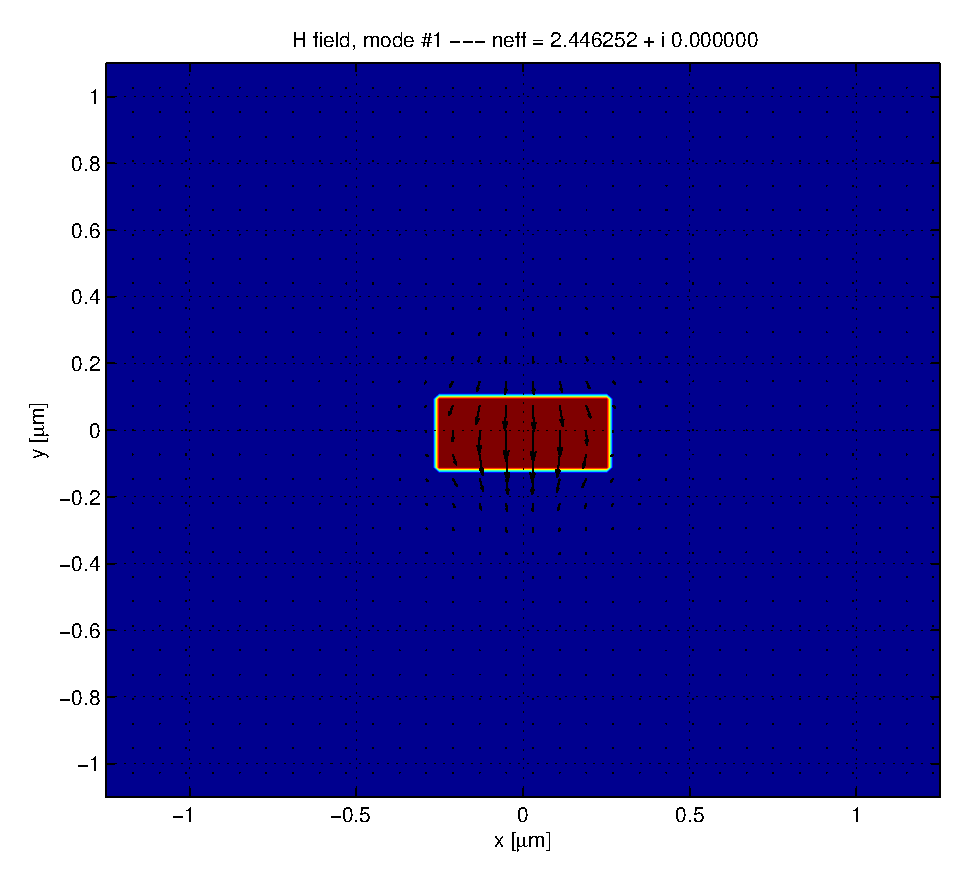
\includegraphics[width=5cm]{pics/plabs_TE1}}
    \subfigure[First TE mode: contourplot of the $H_y$ component.]{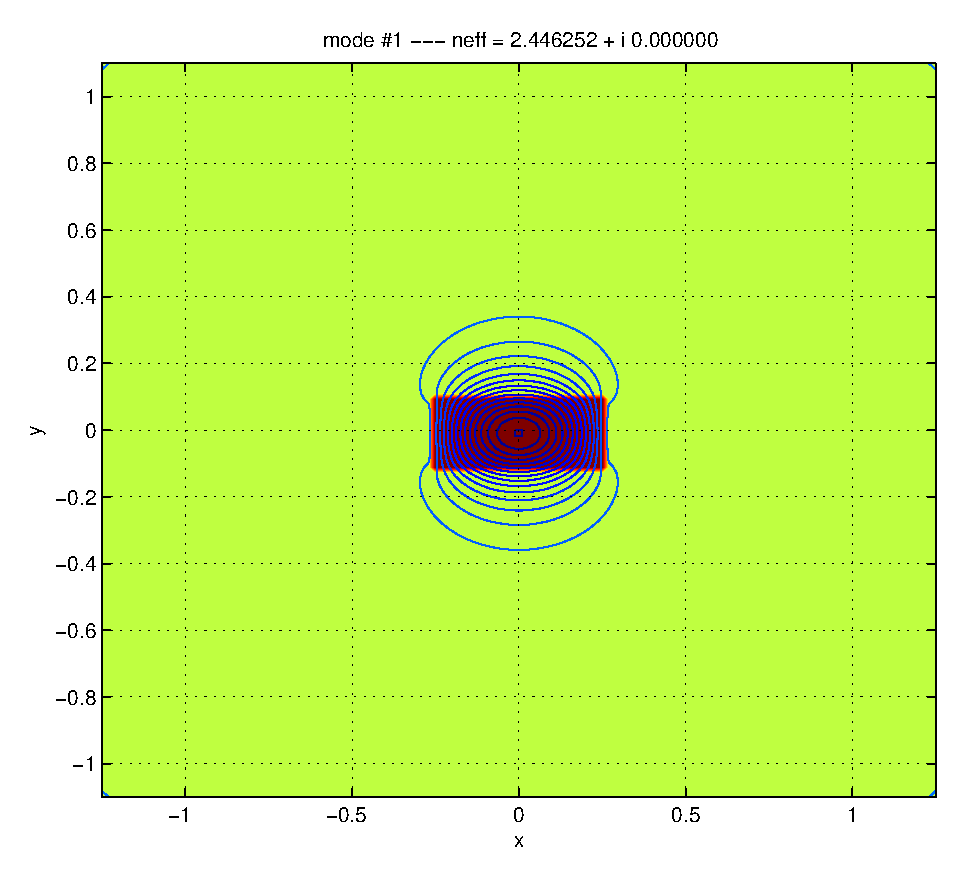
\includegraphics[width=5cm]{pics/plabs_TE1_contour}}
    \subfigure[First TM mode: magnetic field.]{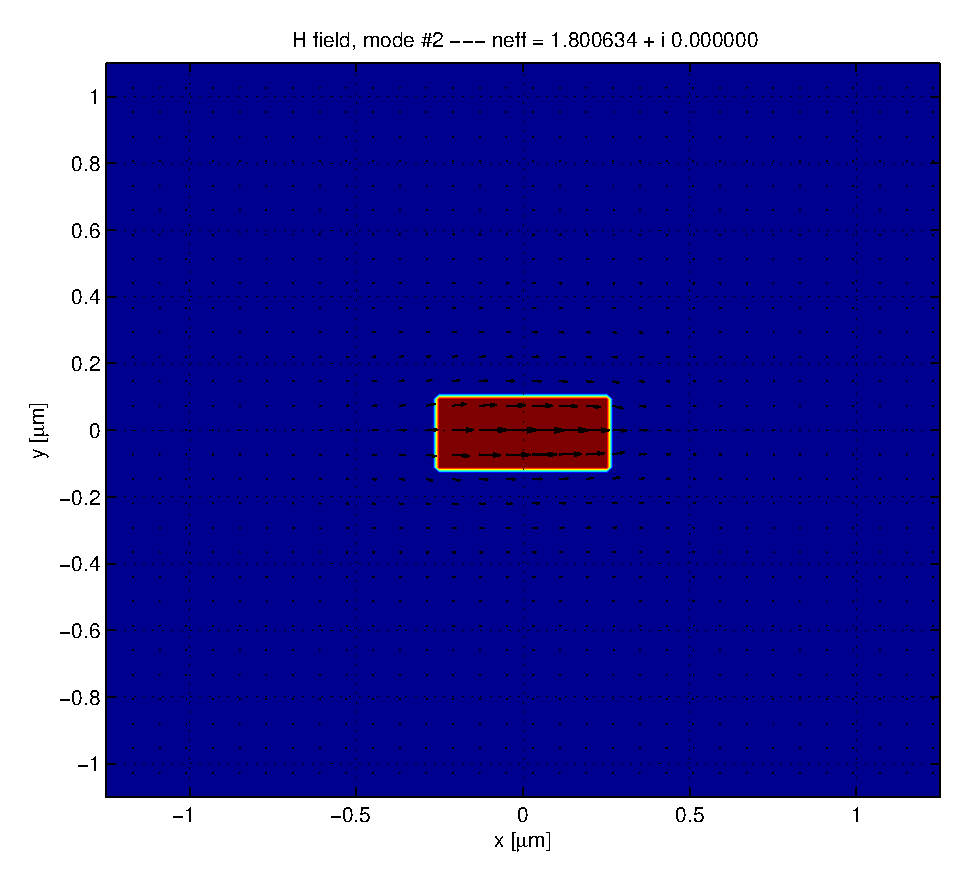
\includegraphics[width=5cm]{pics/plabs_TM1}}
    \subfigure[First TM mode: contourplot of the $H_x$ component.]{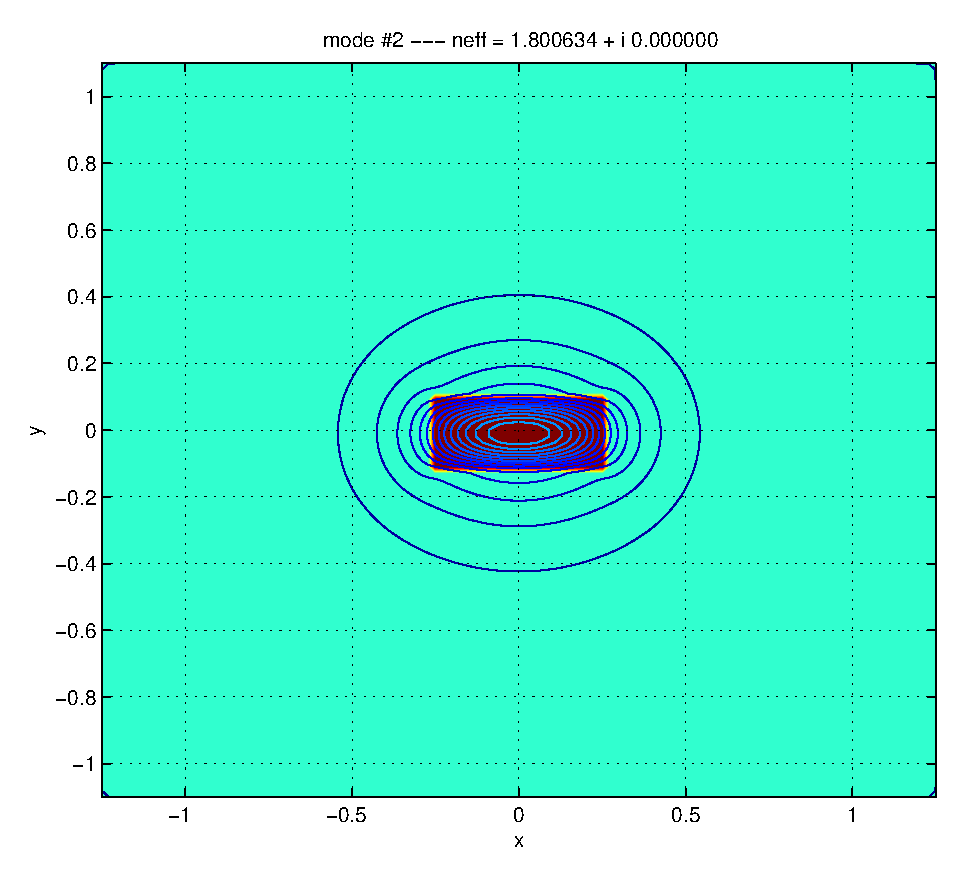
\includegraphics[width=5cm]{pics/plabs_TM1_contour}}
  \end{center}
  \caption{Magnetic field for the first two guided modes.}
  \label{fig:plabs_field}
\end{figure}  

%% \figref{fig:plabs_field} shows the magnetic field for the first two
%% guided modes of the device.

More examples for the use of the vectorial mode solver can be found in
\ref{sec:polrot}.

\OKKIO{fare degli esempi per la convergenza...}
\OKKIO{usare FIMMWAVE come reference??}
